\documentclass[12pt,notitlepage]{article}
\usepackage[bitstream-charter]{mathdesign}
\usepackage{inconsolata}
\usepackage[T1]{fontenc}
\usepackage{microtype}
\usepackage{graphicx}
\usepackage[utf8x]{inputenc}
\usepackage[letterpaper]{geometry}
\usepackage{titlesec}
\usepackage{booktabs}
\usepackage{tabu}
\usepackage{hyperref}

\titleformat{\section}{\normalfont\large}{\thesection}{0.5em}{}
\titleformat{\subsection}{\normalfont}{\thesubsection}{0.5em}{}
\titlespacing*{\section}{0em}{0.75em}{0.3em}

\begin{document}
\begingroup
  \centering
  {\Large Proposal: Concreteness Fading and Visual Programming in
  Teaching Object-Oriented Programming\\[1em]}

  Andy Jiang, Michael Mauer, and David Li\par
\endgroup

\section{Problem Definition}

Much effort has gone towards methods to teach programming as an
overall concept, with systems like Alice, Scratch, and CodeSpells
demonstrating how visual programming can successfully introduce
students to this field. Our goal is to teach the more specific topic
of object-oriented programming to novice programmers using these same
techniques, focusing on how to abstract and represent ideas such as
inheritance, polymorphism, and interfaces in such a framework.
Additionally, to reinforce these concepts to an audience already
somewhat familiar with programming, we will introduce concreteness
fading to the system, transitioning students from visual programming
to directly writing code. This will facilitate the learning of these
specific higher-level concepts and abstractions within computer
science, which is important to effectively educate and train the next
generation of computer science and software development students.

\section{Approach}

Our approach is to develop a game based on visual programming, where
the immediate objective is to manipulate various objects within a
world to accomplish certain goals. Tentatively, the main theme will be
controlling a robot to gather resources, build new robots (teaching
object instantiation, design patterns), writing code for new robots
(teaching inheritance, encapsulation, etc.), or terraforming the
environment. Students will control the robot and other objects via a
block-based visual programming interface akin to Scratch. However, one
novel idea is that the interface will be designed to express
object-oriented concepts, making clear ideas such as method
invocation, object instantiation, and polymorphism. Additionally, the
other novel idea is to use concreteness fading to demonstrate the link
between the abstracted representation and the underlying code: the
system will translate the visual representation to Java code, showing
its execution in tandem with the symbolic execution of the blocks and
the effect of the code in the world. The system will highlight the
visual block being executed, as well as the corresponding line of
code. Eventually, the system will fade the visual representation,
asking students to directly write more and more of the code itself.

Specifically, we intend to integrate various visual metaphors for
object-oriented concepts within the visual programming interface. For
example, class definitions would be represented as ``blueprints''
containing lists of methods, which students would drag into ``tell''
blocks that represent the message-passing style of OOP.\@ Students
would also add an object reference to the ``tell'' block, which the
system would translate into method invocation on the instance. Each
class would have an associated pictorial representation, which would
be attached to object reference blocks in the editor, and which would
also be used to represent instances of that object in the game world
grid. Later on, this representation could be faded by removing the
picture and/or morphing the tell block into the dot syntax used by
Java.

\begin{figure}[h]
  \centering
  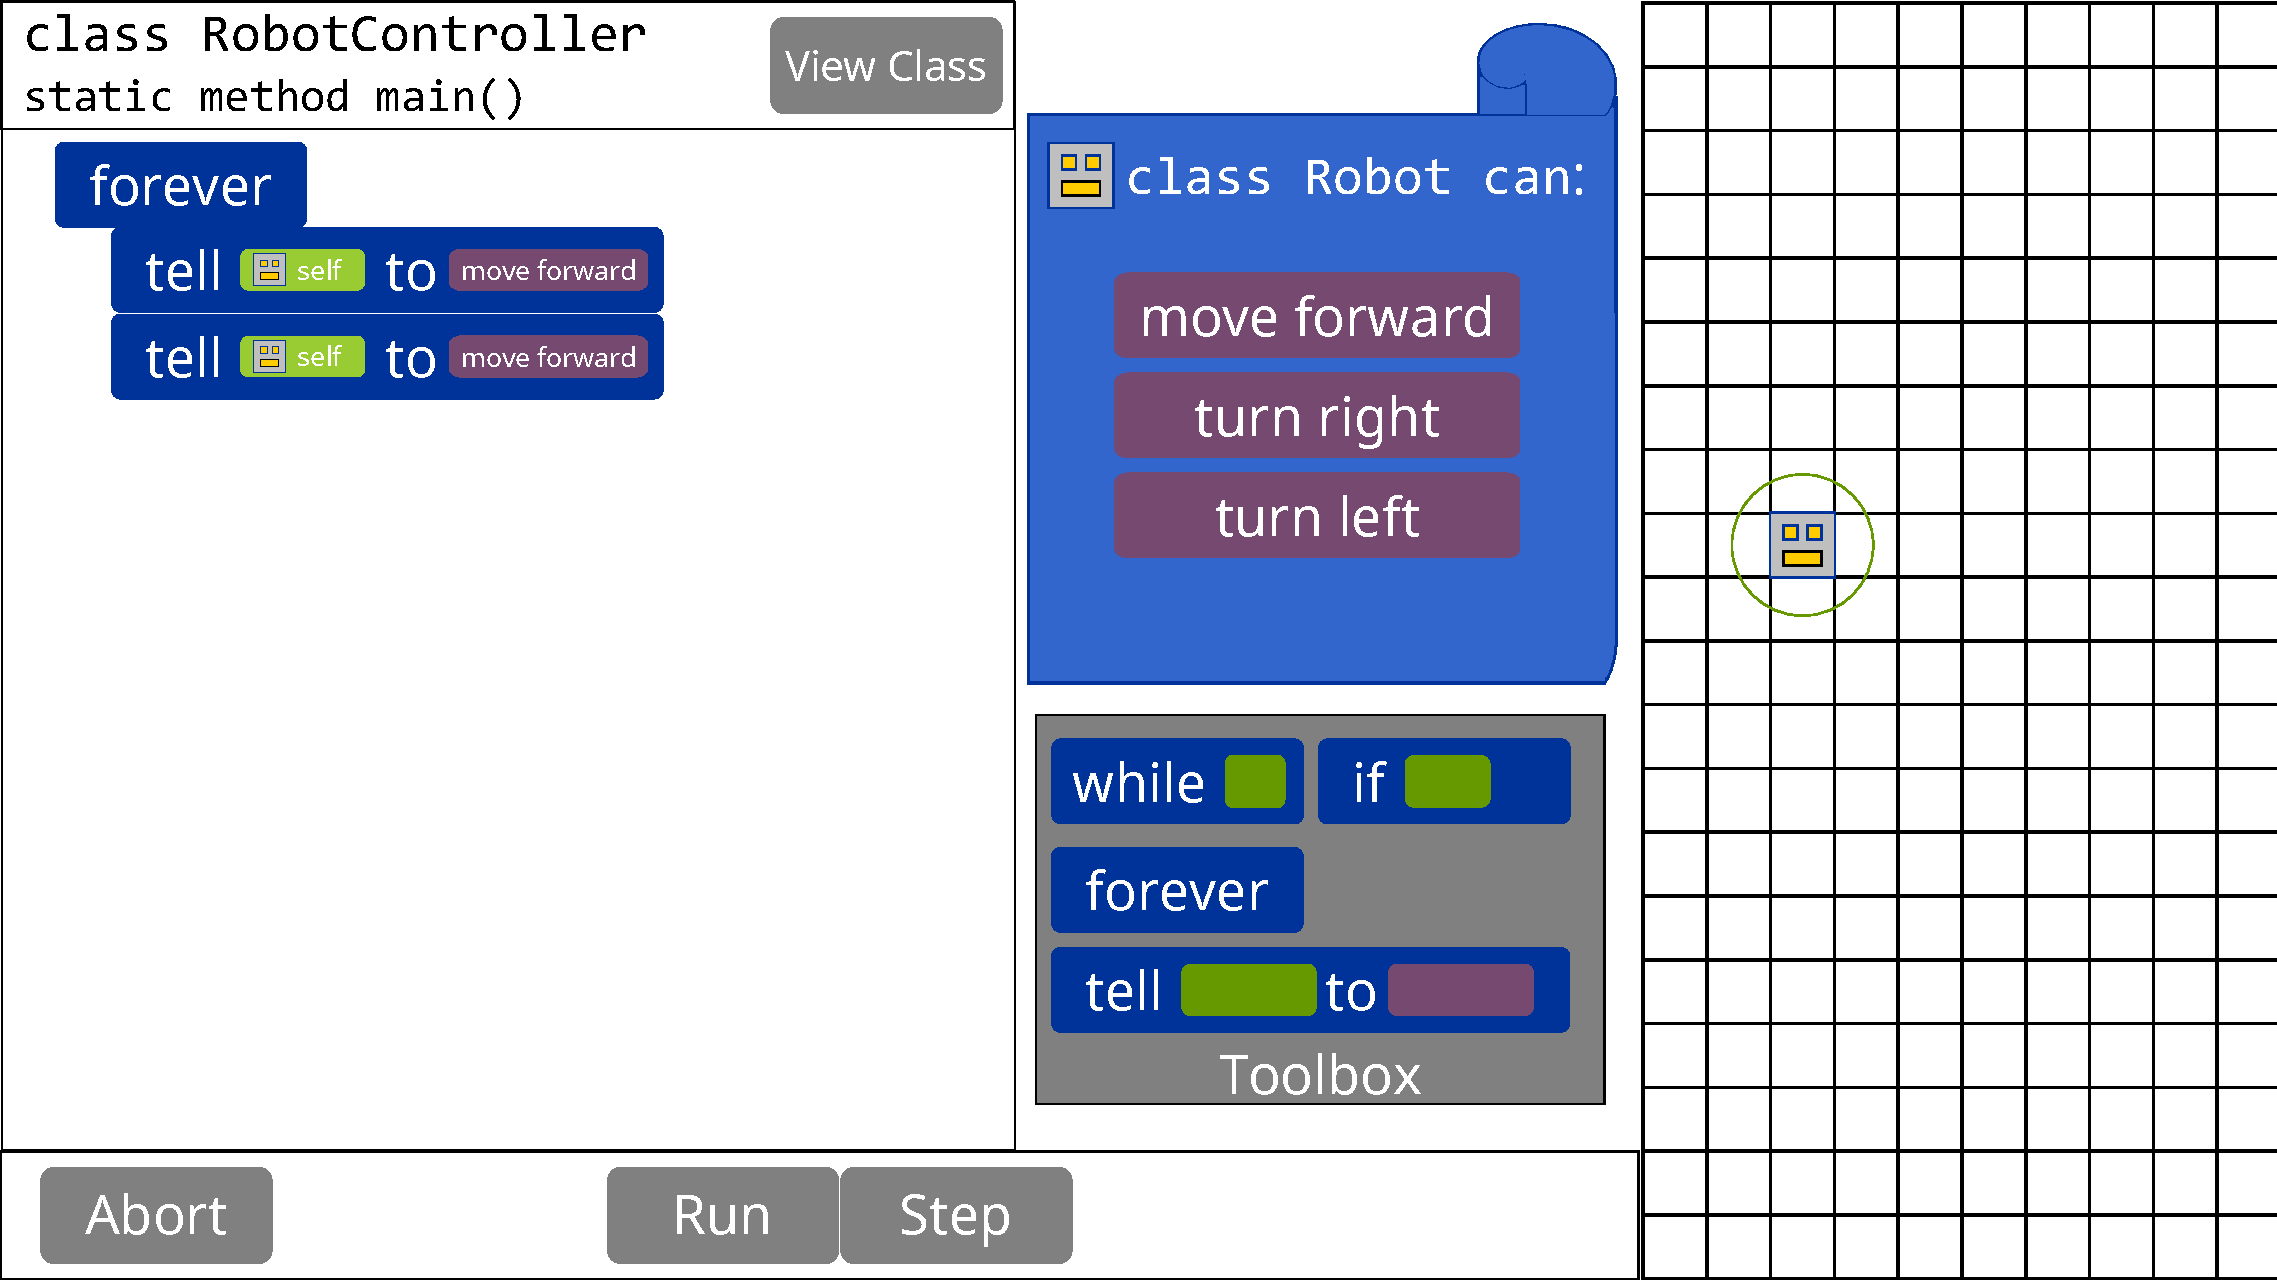
\includegraphics[width=\textwidth]{mockup.pdf}
  \caption{The main game interface.}
\end{figure}

Based on feedback from the paper prototype, the user interface has
been redesigned. There are two main activities: editing code and
executing code. When editing code, the user will have access to the
toolbox of unlocked blocks, an area to assemble them, and a small view
of the world map and objectives. Once the student is done, they will
run the code, at which point the toolbox will shrink, the map will
expand, and the game will begin stepping through their code while
simultaneously displaying their side effects on the world map. We
removed the interactive Java debugger, as students would likely ignore
it. Instead, we plan to fade Java code into the blocks themselves: at
first some blocks will begin displaying code on them; later, some
blocks will be translated into code while executing.

Here the ``blueprint'' metaphor shows the student what methods are
available, and the object instance they are controlling is highlighted
on the map. The \texttt{self} block (\texttt{this} in Java) is
annotated with the same picture as the blueprint and map.

\subsection{Level Design and Progression}

Our rough concept progression can be found in figure~\ref{fig:progression}.

\begin{figure}[h]
  \centering
  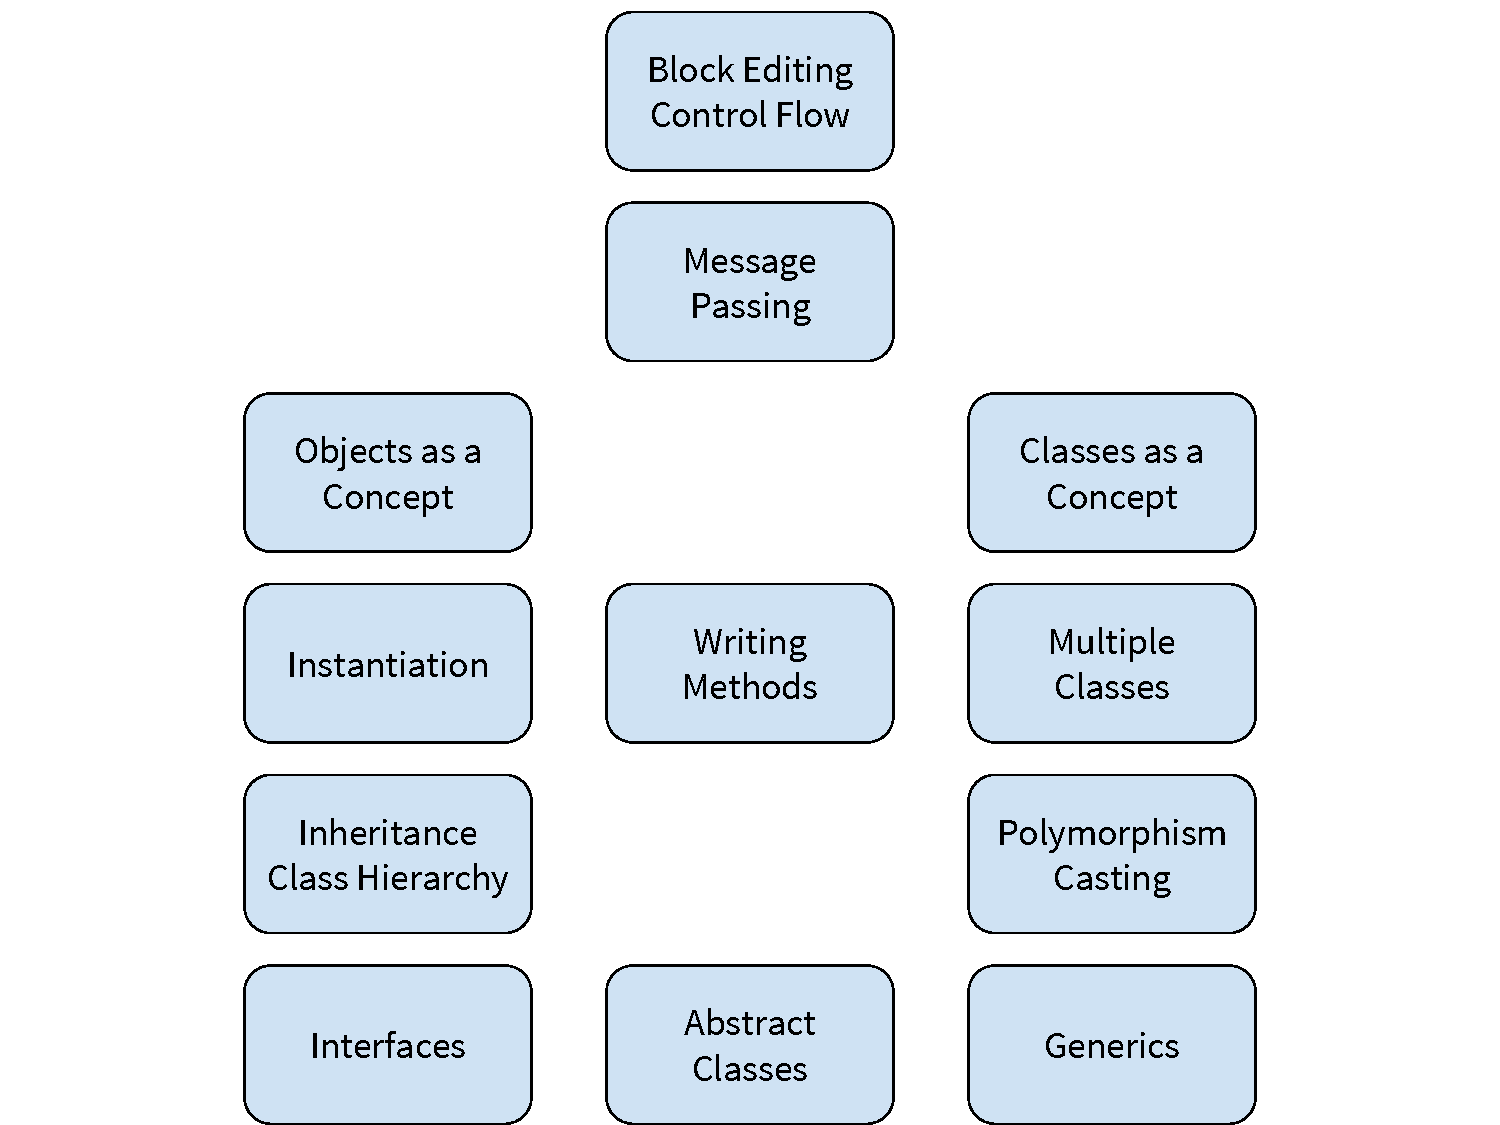
\includegraphics[width=\textwidth]{concept_progression.pdf}
  \caption{The concept progression. Items within a row do not
    necessarily depend on each other, but each row depends on the
    concepts in the previous row.}\label{fig:progression}
\end{figure}

The game will begin and feature a series of interactive
tutorials. When introducing a concept, students will be guided through
using the new idea to accomplish their objectives. In particular, most
block types and capabilities will be slowly introduced, based on
feedback from the paper prototype, where the function and intent of
many blocks was unclear when presented without some sort of
accompanying explanation.

% What are the actions that the player can take in the game? What will
% be the result of these actions?
The actions the player can take, in terms of game mechanics, are
simple: gathering resources, instantiating robots, constructing
buildings in their base, and interacting (via code) with other
environmental objects. Gathering resources allows them to instantiate
more robots/build buildings; buildings may increase the number of
robots they can support or grant access to new types; environmental
objects may advance them in the game's storyline. Overall, the
mechanics here are not intended as an end unto themselves---this is
not a game about gathering minerals and gas. Instead, a set of
objectives will be packaged along with a tutorial and guidance into a
self-contained level, with each level building upon the last.

In terms of editing code, the main actions the user can take are
writing code in the main controller class, which issues commands to
the various robots; defining new methods on robots to implement
various required functionality (e.g.\ being able to control a robot
arm); and defining new robot classes, to make specialized robots for
certain objectives.

% What will the challenges look like?  What will the player
% specifically be asked to do?
As for the challenges themselves, the basic flow will be to:

\begin{enumerate}
\item Instantiate (or be given) new robot(s) in the Controller class
\item Give commands to the robot(s) to:
  \begin{itemize}
  \item Pick up resources
  \item Activate tools to extract resources/terraform
  \item Bring things back to base/a target location
  \item Activate tools to construct buildings
  \item Avoid obstacles/traps
  \end{itemize}
\item Implement new methods and classes, to fill in missing
  functionality or specialize a robot for a task. For instance, the
  robot may not be able to make use of a drill until it is subclassed
  and methods are added to power on the drill, control its speed,
  power it off, etc.
\end{enumerate}

% How will the game increase in difficulty? What will an easy, medium,
% and hard challenge look like?
Some example tasks, with difficulty levels and rationale, are given
below. In general, more difficult tasks involve at least one of the
following: more concepts, more objectives, and less
scaffolding/tutorial material.

\noindent\begin{tabu}{lXX}
  \\
\toprule
Task & Description & Difficulty \\
\midrule
Gathering Iron & Behind a hill and out of sight of the player is
located a deposit of iron. Command the robot to search around the base
of the hill for the iron and bring it back to base.& Easy---this is
primarily about control flow, with method invocations necessary to
command the robot. \\
\\
Two Left Wheels & One of the robots you have can only turn
left. Implement a \texttt{turnRight} method for it. & Easy---this is a
very basic method definition.\\ \\
Robot Rescue & & Medium--- \\ \\
Fracking for Gas & & Medium--- \\ \\
General-Purpose Robot & & Hard--- \\
\bottomrule
\\
\end{tabu}
% How will your game decide whether object-oriented code the player
% has constructed is correct? Will correctness be based purely on
% whether the code performs the desired task, or will you also add
% constraints to enforce object-orientedness? How would this be done?
Our system simply requires the student to accomplish the given
objectives, using the tools given to them. Judging object-orientedness
TODO.

\section{Prior Work}

Compared to prior systems like
Scratch\footnote{\url{https://scratch.mit.edu/}} and
Lightbot\footnote{\url{http://lightbot.com/hour-of-code-2015-flash.html}},
our system will explicitly model object-oriented concepts. For
instance, LightBot provides a fixed set of actions that implicitly
operate on the robot and space for a single subroutine. In contrast,
our system would allow user-defined methods on multiple classes, as
well as multiple different types of objects and control over multiple
objects simultaneously. Compared to Scratch, while our block system is
(intentionally) modeled after theirs, again, our system explicitly
shows the objects and methods being invoked, while in Scratch scripts
are attached to a particular sprite and implicitly act on that
sprite. In other words, while Scratch has all actions take place on
\texttt{this}, our system will show \texttt{this} as well as other
objects and allow the user to manipulate them at will.

Google's Blockly
Games\footnote{\url{https://blockly-games.appspot.com/about},
  \url{https://github.com/google/blockly-games}} demonstrates our
concreteness fading idea: as the game progresses, blocks first have
code appear on them, then the blocks are removed entirely, leaving
only code. Our system differs in that we intend to make this
transition between blocks and code gradually, migrating the blocks to
show code on them slowly, then having some tasks (e.g.\ the
implementation of some methods) be code-only, before ending with
code-only.

\section{Evaluation}

We intend to test the system with a group of students in a class such
as CS 2110, Advanced Placement Computer Science, or similar class
involving Java and object-oriented principles. Students could be given
a pre- and post- test asking about various concepts from this
paradigm. As noted from feedback on the paper prototype, finding an
appropriate target audience is difficult---we need students who have
some programming basics, but who have not fully learned OOP.\@ TODO:
solution.

As for other data to collect, we can record basic statistics such as
the amount of time spent in the game, the amount of time per lesson,
the number of tries per lesson, and so on. We could also record their
intermediate attempts at a solution.

\section{Milestones}

\subsection{Alpha}

The minimum playable product would require:
\begin{itemize}
\item Block editor
\item World map
\item Code execution
\item The first lesson
\end{itemize}

\begin{tabu}{Xlll}
\toprule
Task & Priority & Person & Hours \\
\midrule
Integrate Google Blockly as the block editor & Must have & Person & Hours \\
Set up Blockly to generate Java code & Must have & Person & Hours \\
Find art assets for the world map & Must have & Person & Hours \\
Render the map using Phaser.js & Must have & Person & Hours \\
Implement ``shim'' classes, to be called by the player code, which update the game state & Must have & Person & Hours \\
Implement the game state & Must have & Person & Hours \\
Relay the game state via WebSocket to the client & Must have & Person & Hours \\
Step through Java code using the Java Debug Interface & Must have & Person & Hours \\
Relay code execution events via WebSocket to the client & Must have & Person & Hours \\
\bottomrule
\end{tabu}

\subsection{Beta}

\begin{itemize}
\item Level creation tools (to develop content and lessons quickly)
\item Tutorial/hint capability (to guide players through a lesson)
\item More lessons
\item Savegame capability
\end{itemize}

\begin{tabu}{lXXl}
\toprule
Task & Priority & Person & Hours \\
\midrule
Task description & Must/should/could have & Person & Hours \\
\bottomrule
\end{tabu}

\subsection{Final}
\begin{itemize}
\item All the lessons, covering up to subclassing/class hierarchy (our
  target concept)
\item Data collection
\end{itemize}

\begin{tabu}{lXXl}
\toprule
Task & Priority & Person & Hours \\
\midrule
Task description & Must/should/could have & Person & Hours \\
\bottomrule
\end{tabu}

\end{document}
